\documentclass{article}
\usepackage{geometry}
\geometry{paperwidth=21cm,
paperheight=29.7cm,
margin=1cm}
\usepackage{amsmath}
\usepackage{mathfmv}
\usepackage{siunitx}
\usepackage{pgf}
\usepackage{tikz}
\usepackage{pgfplots}
\pgfplotsset{compat=1.18}
\begin{document}
\[
\boldsymbol{H(p)=2\dfrac{p+1}{0.05p^3+0.6p^2+p}}
\]
\begin{center}
\begin{tikzpicture}[trim axis left]
\begin{axis}[ticklabel style = {font=\normalsize},
width=0.9\textwidth,
height=0.25\textheight,
grid=both,
major grid style={black!40},
label style={font=\large},
xmode=log,ymode=normal,
xlabel={},
ylabel={Gain (\si{\decibel})},
xtick={0.01,0.1,1.0,10.0,100.0},
ytick={-40,-32,-24,-16,-8,0,8,16,24,32,40},
xticklabels={$10^{-2}$,$10^{-1}$,$10^{0}$,$10^{1}$,$10^{2}$},
yticklabels={-40,-32,-24,-16,-8,0,8,16,24,32,40},
xmin=0.01,xmax=100.0,
ymin=-40,ymax=40]
\addplot[ultra thick, blue,domain=0.01:100.0,samples=256]{32.04119982655925+10*log10(1.0+(x+(0.0))*(x+(0.0)))-20*log10(x)-10*log10(99.99999999999997+(x+(0.0))*(x+(0.0)))-10*log10(4.000000000000002+(x+(0.0))*(x+(0.0)))};
\addplot[line width=2pt,red,dashed,domain=0.01:1.0, samples=16]{6.020599913279624-20*log10(x)};
\addplot[line width=2pt,red,dashed,domain=1.0:2.0000000000000004, samples=16]{6.020599913279624-20*log10(x)+(20.0)*log10(x/1.0)};
\addplot[line width=2pt,red,dashed,domain=2.0000000000000004:9.999999999999998, samples=16]{6.020599913279624-20*log10(x)+(20.0)*log10(x/1.0)+(-20.0)*log10(x/2.0000000000000004)};
\addplot[line width=2pt,red,dashed,domain=9.999999999999998:100.0, samples=16]{6.020599913279624-20*log10(x)+(20.0)*log10(x/1.0)+(-20.0)*log10(x/2.0000000000000004)+(-20.0)*log10(x/9.999999999999998)};
\end{axis}
\end{tikzpicture}

\begin{tikzpicture}[trim axis left]
\begin{axis}[ticklabel style = {font=\normalsize},
width=0.9\textwidth,
height=0.25\textheight,
grid=both,
major grid style={black!40},
label style={font=\large},
xmode=log,ymode=normal,
xlabel={Pulsation (\si{\radian\per\second})},
ylabel={Phase (\si{degree})},
xtick={0.01,0.1,1.0,10.0,100.0},
ytick={-180,-162,-144,-126,-108,-90,-72,-54,-36,-18,0},
xticklabels={$10^{-2}$,$10^{-1}$,$10^{0}$,$10^{1}$,$10^{2}$},
yticklabels={-180,-162,-144,-126,-108,-90,-72,-54,-36,-18,0},
xmin=0.01,xmax=100.0,
ymin=-180,ymax=0]
\addplot[ultra thick, blue,domain=0.01:100.0,samples=256]{-90+(1)*atan2(x/1.0,1)+(-1)*atan2(x/2.0000000000000004,1)+(-1)*atan2(x/9.999999999999998,1)};
\addplot[line width=2pt,red,dashed,domain=0.01:1.0,samples=16]{-90};
\draw[line width=2pt,red,dashed](axis cs:1.0,-90) -- (axis cs:1.0,0.0);
\addplot[line width=2pt,red,dashed,domain=1.0:2.0000000000000004,samples=16]{0.0};
\draw[line width=2pt,red,dashed](axis cs:2.0000000000000004,0.0) -- (axis cs:2.0000000000000004,-90.0);
\addplot[line width=2pt,red,dashed,domain=2.0000000000000004:9.999999999999998,samples=16]{-90.0};
\draw[line width=2pt,red,dashed](axis cs:9.999999999999998,-90.0) -- (axis cs:9.999999999999998,-180.0);
\addplot[line width=2pt,red,dashed,domain=9.999999999999998:100.0,samples=16]{-180.0};
\end{axis}
\end{tikzpicture}
\end{center}
\paragraph{Fonctions réelles du gain et du déphasage}
\[
G(\omega)=|H(\jw)|=\dfrac{40\left(j \omega + 1\right)}{- \frac{j \omega^{3}}{20} - \frac{3 \omega^{2}}{5} + j \omega}
\]
\[
G_{dB}(\omega)=32+10\log{\left(1+\left(\frac{\omega}{\omega_1}\right)^2\right)}+20\log\omega-10\log{\left(1+\left(\frac{\omega}{\omega_2}\right)^2\right)}-10\log{\left(1+\left(\frac{\omega}{\omega_3}\right)^2\right)}
\]
\[
\phi(\omega)=\arg{H(\jw)}=-90+\arctan{\left(\frac{\omega}{\omega_1}\right)}-\arctan{\left(\frac{\omega}{\omega_2}\right)}-\arctan{\left(\frac{\omega}{\omega_3}\right)}
\]
\paragraph{Quelques valeurs particulières calculées}
\begin{center}
\begin{tabular}{ccc}
\hline
$\omega$ (\si{\radian\per\second}) & Gain (\si{\decibel}) & Phase (\si{\degree})\\
\hline
     0.01000 &     46.02092 &    -89.77083\\
\hline
     0.02512 &     38.02258 &    -89.42458\\
\hline
     0.06310 &     30.03333 &    -88.55813\\
\hline
     0.15849 &     22.10008 &    -86.43306\\
\hline
     0.39811 &     14.48389 &    -81.82971\\
\hline
\textbf{     1.00000} & \textbf{     8.01859} & \textbf{   -77.27564}\\
\hline
\textbf{     2.00000} & \textbf{     3.80907} & \textbf{   -82.87498}\\
\hline
     2.51189 &      2.28199 &    -87.28087\\
\hline
     6.30957 &     -5.72227 &   -113.66853\\
\hline
\textbf{    10.00000} & \textbf{   -11.09622} & \textbf{  -129.40066}\\
\hline
    15.84893 &    -17.46556 &   -144.16793\\
\hline
    39.81072 &    -32.23273 &   -164.46259\\
\hline
   100.00000 &    -48.00332 &   -173.71658\\
\hline
\end{tabular}
\end{center}
\end{document}
